%% Bemærk:
%%          Resten af rapporten følger en stil hvor indledninger skrives
%%          med \sffamlily-typen. Denne stil bør også følges her.
%%
{\sffamily
I denne sektion vil vi test den udvidet løsning, om den virker som vi
hade planlagt på test billeder og om hvordan den virker i praktisk på
udvalgte malerier.
}
\subsection{Afprøvning på testbilleder}
Vi teste metoden på 4 test billeder. Billedet \ref{hus_virker} er et hus
hvor snittet og massemidtpunktet næsten ligge oven i hinanden. 

\begin{figure}[h!!]
	\begin{center}
		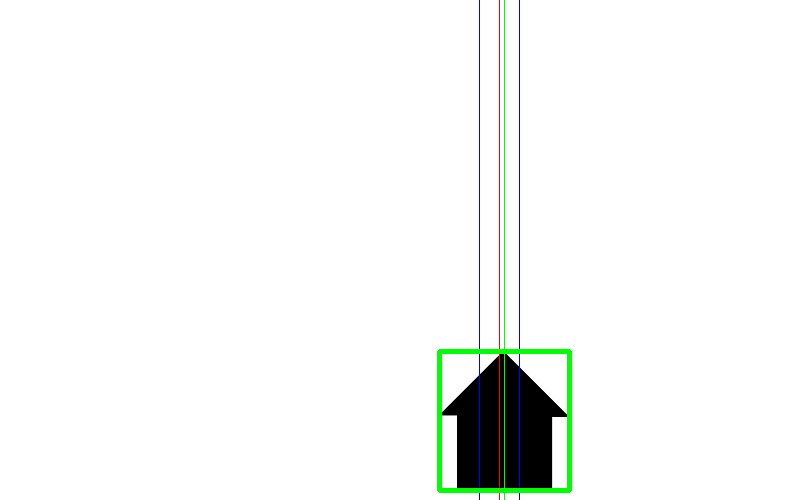
\includegraphics[scale=0.3,angle=0]{afsnit/afprovning/billeder/udvidet_losning/udvidet_hus1_test.png}
	\end{center}
	\caption[]{Et hus der er symetrisk og der har massemidtpunkt i spisen af taget, massemidtpunktet er inde for margin så huset bliver udvalgt til at ligge i snittet.}
	\label{hus_virker}
\end{figure}

I det andet billedet \ref{hus_virker_ikke} er huset forskubbet så masse
midtpunktet lige lige uden for margin, og derved ikke skulle blive tage
med af algoritmen. 

\begin{figure}[h!!]
	\begin{center}
		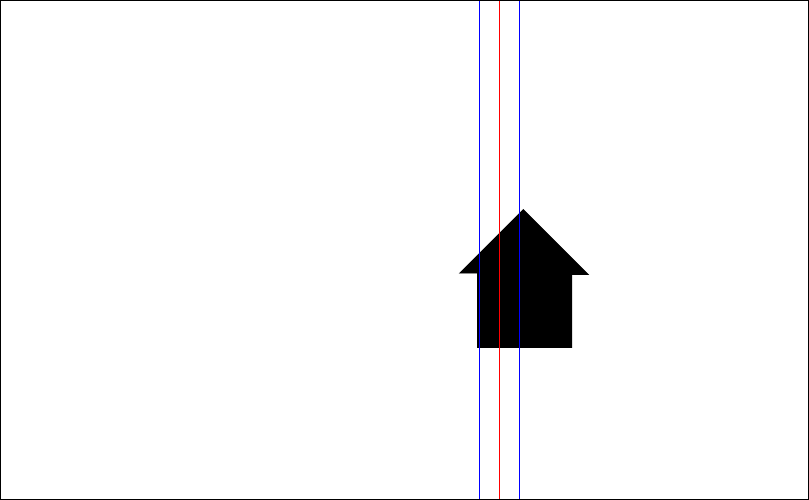
\includegraphics[scale=0.3,angle=0]{afsnit/afprovning/billeder/udvidet_losning/udvidet_hus2_test.png}
	\end{center}
	\caption[]{Hus hvor masse midtpunktet er flyttet få pixels ud for margin, den udvide løsning vælger ikke at tage huset med.}
	\label{hus_virker_ikke}
\end{figure}

Det tredje billedet \ref{udvidet_blob_test} har en region som er meget lille
og derfor bliver fra sorteret på grund af den størrelse, den stor
region, bliver taget med at dens massemidtpunkt ligger inden for margin. 

\begin{figure}[h!!]
	\begin{center}
		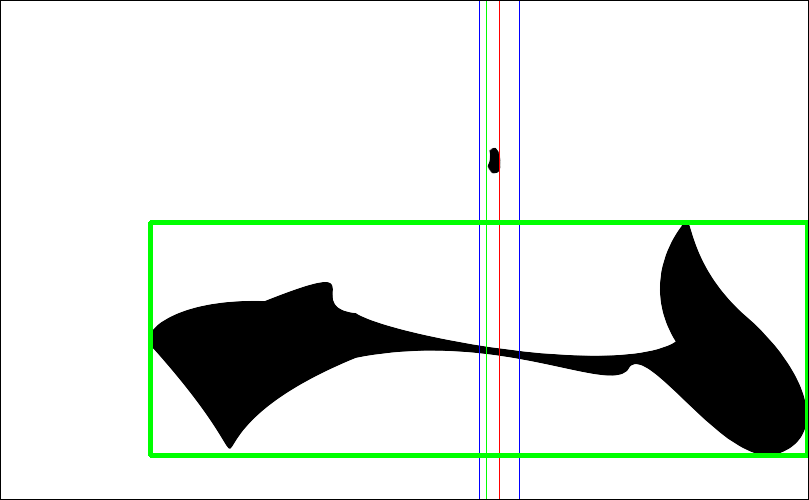
\includegraphics[scale=0.3,angle=0]{afsnit/afprovning/billeder/udvidet_losning/udvidet_blob2_test.png}
	\end{center}
	\caption[]{2 regioner hvor den nederste har et massemidtpunkt inde for margin.}
	\label{udvidet_blob_test}
\end{figure}

Det fjerre billedet \ref{bleksprutte_test} er der en region med som har
et massemidtpunkt inde i margin, men som har en skæv fordeling af pixels
i forhold til snittet og derfor bliver sorteret fra. Ud fra de fire
observationer, virker det som om, den udvidet løsning virker efter
forventningerne.

\begin{figure}[h!!]
	\begin{center}
		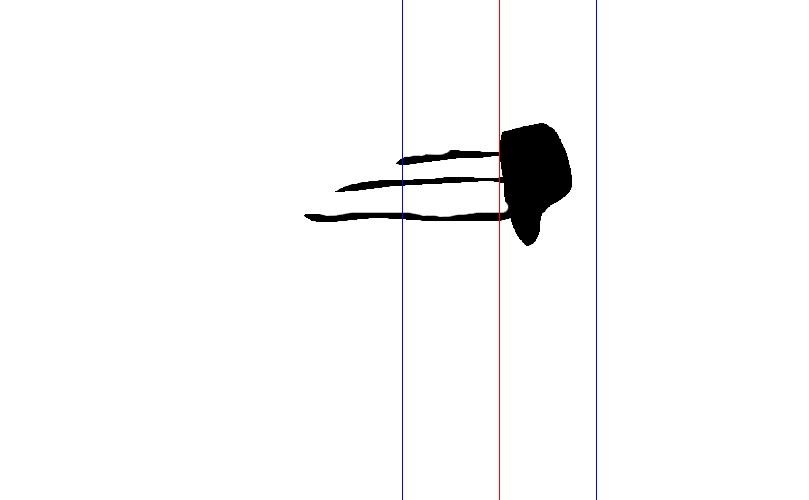
\includegraphics[scale=0.3,angle=0]{afsnit/afprovning/billeder/udvidet_losning/udvidet_bleksprutte_test.png}
	\end{center}
	\caption[]{Margin er sat meget op, så man kan se at regionen har et massemidtpunkt ind for margin, men da størstedelen af regionens pixels er på højre side, vælger den fra.}
	\label{bleksprutte_test}
\end{figure}

Som man kan se af testbillederne vælger den udvidet løsning vid
forskellige regioner til at ligger i snittet. 
\clearpage


\subsection{Afprøvning på malerier}
Afprøvningen af den udvidet løsning på malerier fra vores database,
foregå på samme måde som den naive test.

\begin{figure}[h!!]
	\begin{center}
		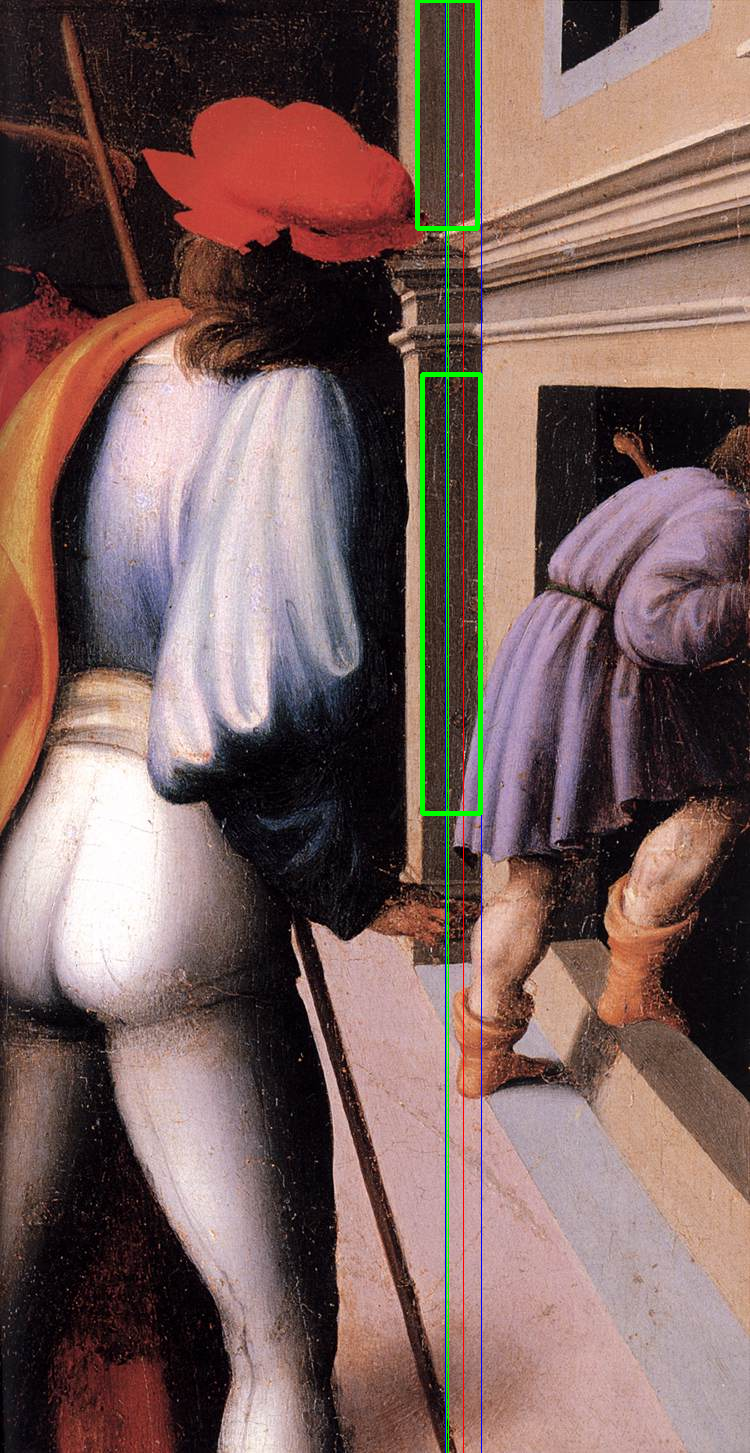
\includegraphics[scale=0.3,angle=0]{afsnit/afprovning/billeder/udvidet_losning/udvidet_kfarver_sdetaljer.png}
	\end{center}
	\caption[]{2 ud af de 6 region er godtager som ligene i det gyldne snit af den udvidet løsning}
	\label{udvidet_virker1}
\end{figure}

\begin{figure}[h!!]
	\begin{center}
		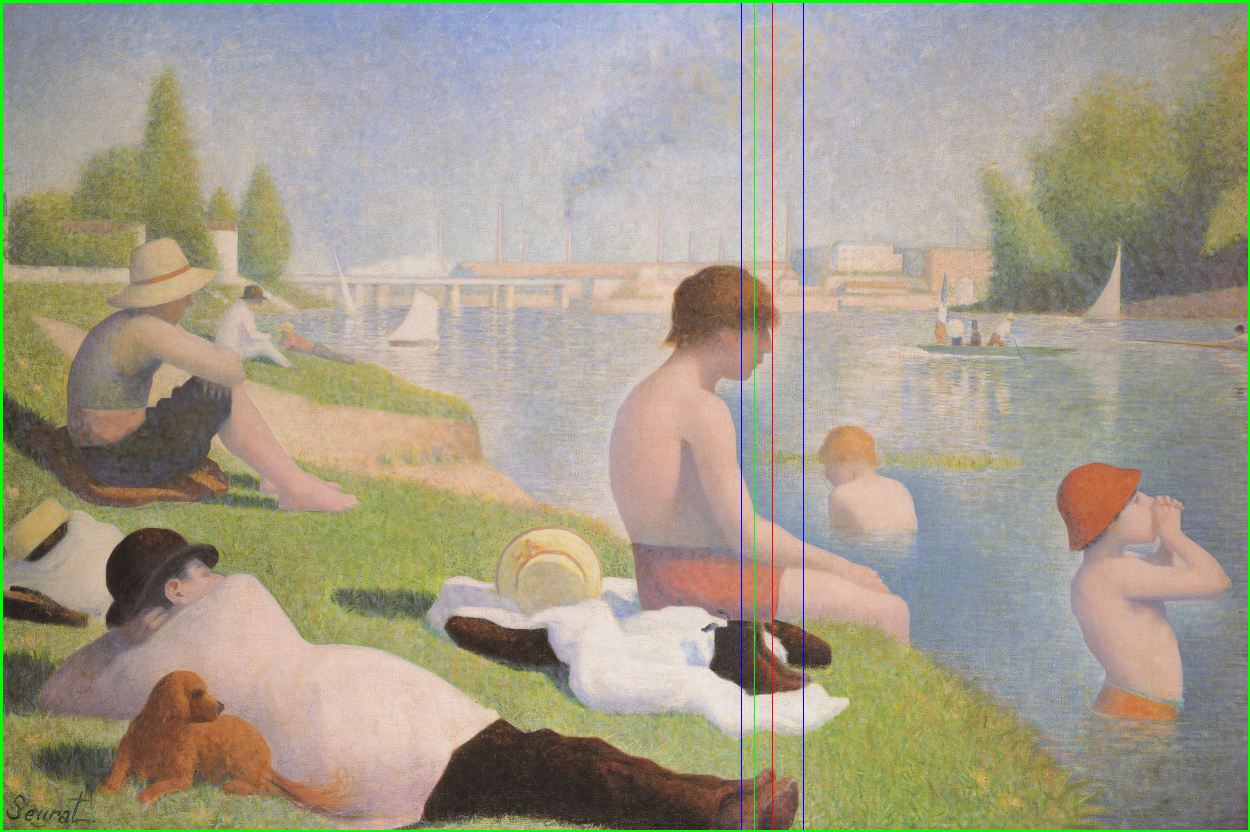
\includegraphics[scale=0.3,angle=0]{afsnit/afprovning/billeder/udvidet_losning/udvidet_dreng.png}
	\end{center}
	\caption[]{baggrunden er den nedeste region som bliver godtaget, da den har et massemidtpunkt som liger inde for marginen}
	\label{udvidet_virker2}
\end{figure}

\begin{figure}[!h]
    \centering
    	\subfloat[Udvidet løsning]{
        	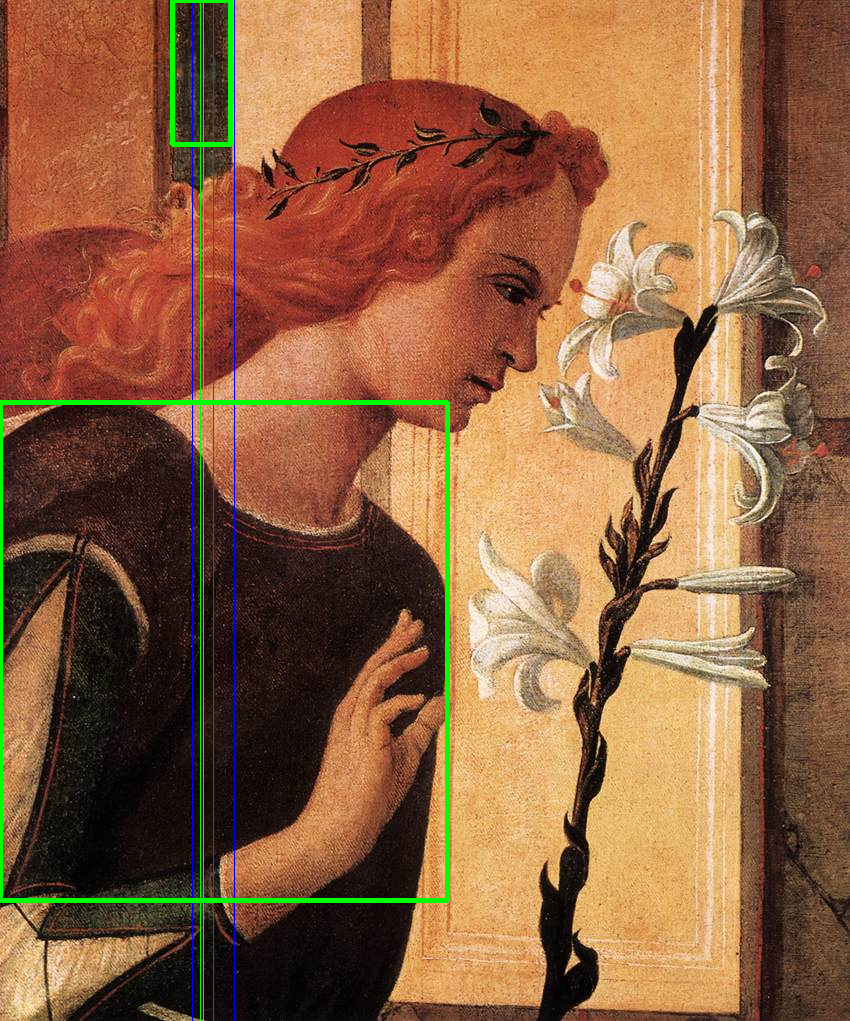
\includegraphics[angle=0,width=0.45\textwidth]{afsnit/afprovning/billeder/udvidet_losning/udvidet_pige.png}
        	\label{udvidet_pige}}\hspace{1em}
    	\subfloat[naiv løsning]{
        	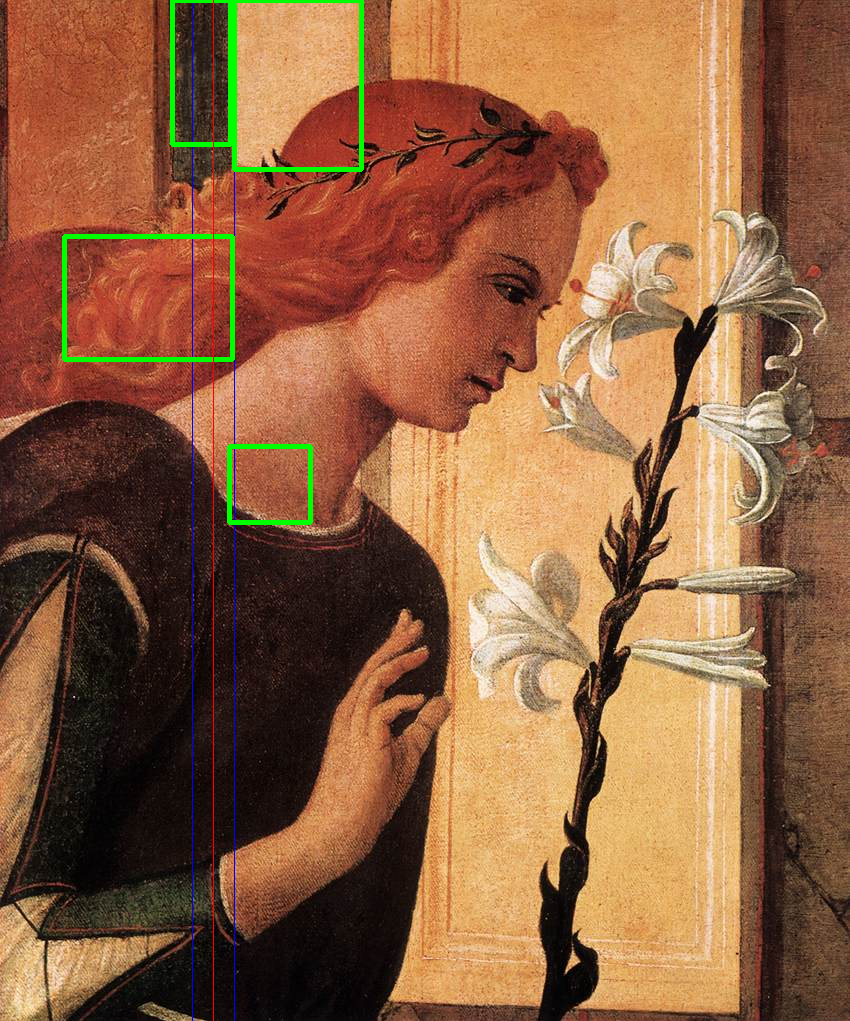
\includegraphics[angle=0,width=0.45\textwidth]{afsnit/afprovning/billeder/udvidet_losning/naiv_pige.png}
        	\label{naiv_pige}}\hspace{1em}        	    			
        \caption[]{Et maleri hvor resultatet for den udvidet og den naive løsning er protrateret. Der bliver fundet forskellige regioner for vær af algoritmerne. Navn: Angel Announcing. År ca. 1500. Af: Bellini, Giovanni}
     \label{udvidet_virker3}
\end{figure}

\begin{figure}[h!!]
	\begin{center}
		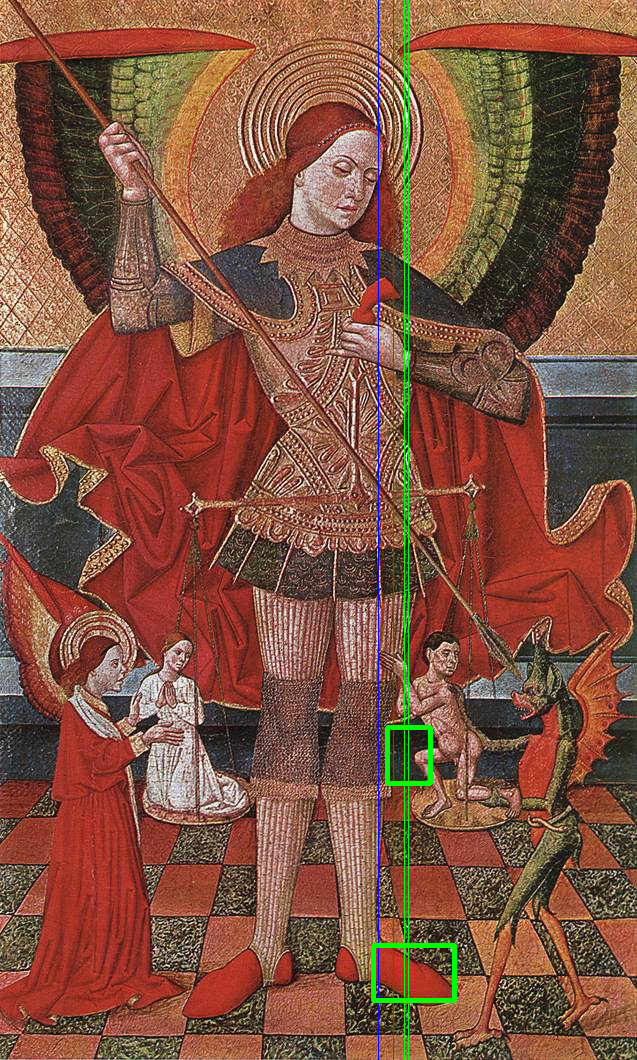
\includegraphics[scale=0.3,angle=0]{afsnit/afprovning/billeder/udvidet_losning/udvidet_kfarver_kdetaljer.png}
	\end{center}
	\caption[]{En sko og en flise bliver taget med at algoritmen}
	\label{udvidet_virker_ikke1}
\end{figure}

\begin{figure}[h!!]
	\begin{center}
		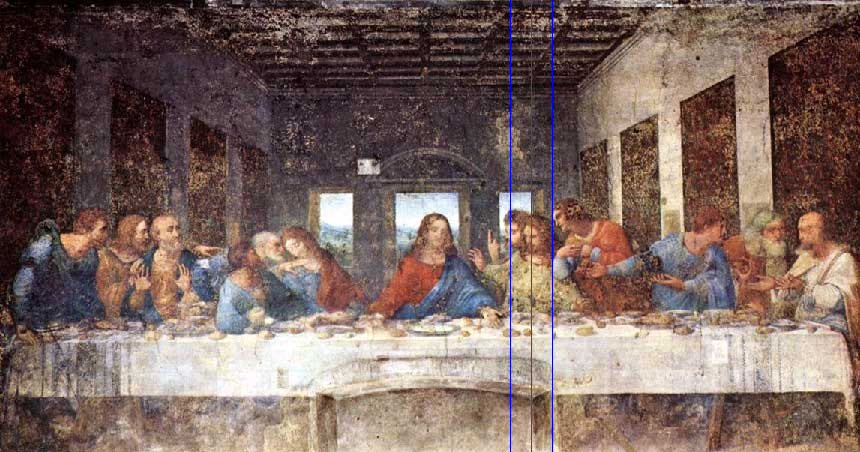
\includegraphics[scale=0.3,angle=0]{afsnit/afprovning/billeder/udvidet_losning/udvidet_mfarver_mdetaljer.png}
	\end{center}
	\caption[]{Den udvidet løsning sortere alle regioner væk}
	\label{udvidet_virker_ikke2}
\end{figure}

\begin{figure}[h!!]
	\begin{center}
		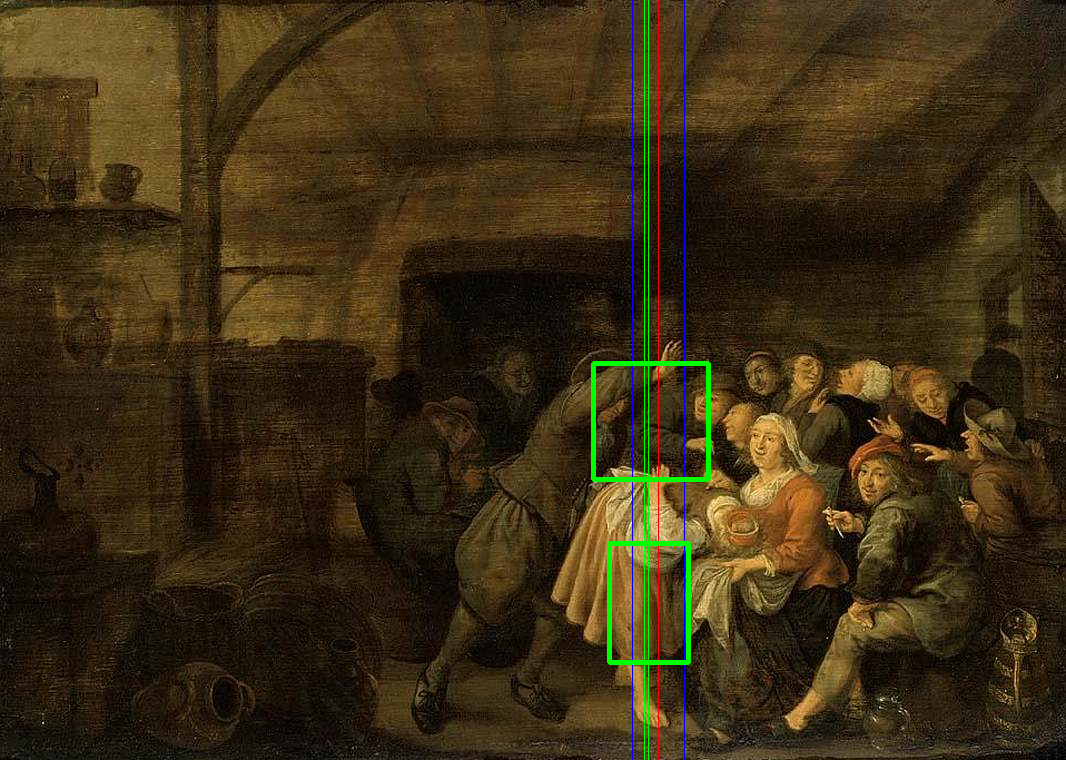
\includegraphics[scale=0.3,angle=0]{afsnit/afprovning/billeder/udvidet_losning/udvidet_sfarver_mdetaljer.png}
	\end{center}
	\caption[]{2 regioner som ikke høre nogle steder hende bliver fundet}
	\label{udvidet_virker_ikke3}
\end{figure}
\clearpage

\subsection{Konklusion}
Ud for teste billederne ser det ud til at den udvidet metode virker på
den måde som vi havde planlangt at den skulle virke. I den praktiske
brug på malerierne, finder den udvidet løsning mange gode regioner hvis
regions detektoren virker se figur \ref{udvidet_virker1}, men kommer
desværre stadig med få regioner som ikke er særlige gode, f.eks i maleri
\ref{udvidet_virker2}. Der udvidet løsning finder også regioner som den
naive ikke vil finde se en sammenlining i figur \ref{udvidet_virker3}. I
de tilfælde hvor regions detektoren ikke virker godt, er den udvide
løsning god til at sorter regioner væk og kommer derfor ikke med særlige
mange regioner som ikke skulle være der, se figur
\ref{udvidet_virker_ikke2} og \ref{udvidet_virker_ikke3}. Dog kommer vi
stadig ud i problemer, hvor der kun er regioner som er forkerte med,
se figur \ref{udvidet_virker_ikke1}.
